% !TEX root = main.tex
\section{Context of the study}\label{sec:context}


This work is carried out in the context of ... {\bf anonymized for the double blind review.}
%the {\em Next-Generation Electrical Architecture (NGEA)} and {\em Next-Generation Electrical Architecture - step 2 (NGEA2)} projects, funded by Vinnova~\cite{Vinnova}. 
%These projects are coordinated by Volvo Cars and involve the Chalmers University of Technology, some research centers in Sweden and many suppliers of the OEM, including Autoliv, Arccore, Combitech, Cybercom, Knowit, Prevas, \AA F-Technology, Semcom, and Qamcom. The projects aim to develop new software processes and proof of concepts to strengthen the competitiveness of the automotive industry in Sweden. 
To this aim, the projects investigate (i) the transition of \company{} %Volvo Cars 
towards CI\&D, (ii) new business models and innovative ways of working within the automotive %\chg{ecosystem}{
value-chain, %}, 
and (iii) vehicles as part of a system of systems. 
%Included in this project are sub projects or work packages that focus on 1) management, administration and business intelligence studies, 2) continuous deployment of architectural and development strategic viewpoints, and 3) automobiles as a system within an automotive software ecosystem \cite{Vinnova}. 
In this paper we mostly focus on point (ii) %\chg{even though there will be some impact on point~(i)}{
and its impact on (i). %}. 
With the increasing transformation of OEMs into software companies, software engineering competences become increasingly crucial, too.
%Since OEMs are increasingly transforming into software companies, the automotive domain is attracting the attention of the software engineering community.  
%\todo{why relevant for ICSE?}

%\ins
{In this paper, we refer to software-related, }%\del{The automotive ecosystem consists of}
inter-organizational collaborations between automotive suppliers %\ins
{and manufacturers (the OEMs) as \emph{automotive ecosystem}}. %\del{It}\ins
%\chg{{This} is characterized by relying on complex supplier networks and strong dependence on hardware and software development~\cite{Knauss2014d}.
%The current automotive industry is {\em closed}, with strict organizational boundaries, stiff processes, established business models, and a straightforward value creation~\cite{ConnectedVehicle2012}.}
%{
Perceived as an ecosystem, the current automotive industry can be characterized as \emph{closed}, with strict organizational boundaries, stiff processes, established business models, and a straightforward value creation \cite{ConnectedVehicle2012}.
Yet, it relies on complex supplier networks  and strong dependence on hardware and software development~\cite{Knauss2014d}. %}


Nowadays, a vehicle is a {\em driving software package} as compared to the vehicles of not even ten years ago. J\"orgen M\"ossinger, VP for automotive systems integration at Bosch, said: ``Electronics and especially software are the main sources of automotive innovation today."~\cite{Mossinger2010SoftwareAutomotive}. The Boston Consulting Group estimates that the total costs of electronic parts will rise from 20\% of the value in a typical car in 2004 to 40\% in 2015. Software, instead of hardware, has become the differentiating factor% of products
~\cite{ConnectedVehicle2012,hbr2015hardwaresoftware,Mossinger2010SoftwareAutomotive,Broy:2006:CAS:1134285.1134292} %. In the past, hardware was the differentiator 
between companies and their products. This evolution of the automotive industry, illustrated by the exponential increase of software, creates new challenges regarding software integration, development, deployment, and maintenance. Therefore, its development needs to support the related integration and evolution over time~\cite{Broy:2006:CAS:1134285.1134292,qualman2009socialnomics,JansenTale2009}. The increasing number of stakeholders involved in the software development projects imposes additional challenges to the architecture teams, as software development and design literally cannot be controlled, or even understood, in detail by a single group any more. 

%\chg{The}
Key stakeholders in the automotive value-chain are classified as OEMs (e.g. \company{}) and their suppliers (Tier-1 and Tier-2). 
In general, an OEM is the coordinator and platform owner in the automotive ecosystem~\cite{KS15}. 
Tier-1 suppliers are considered as direct suppliers to OEM and Tier-2 companies are a second level of suppliers, indirect to the OEM and directly connected to Tier-1. 
% and vice versa, hence, indirect to the OEM. \todo{is this relevant+understandable by ICSE readers?}

%\begin{figure}[htb]
%\vspace{-.2cm}
%\centering
%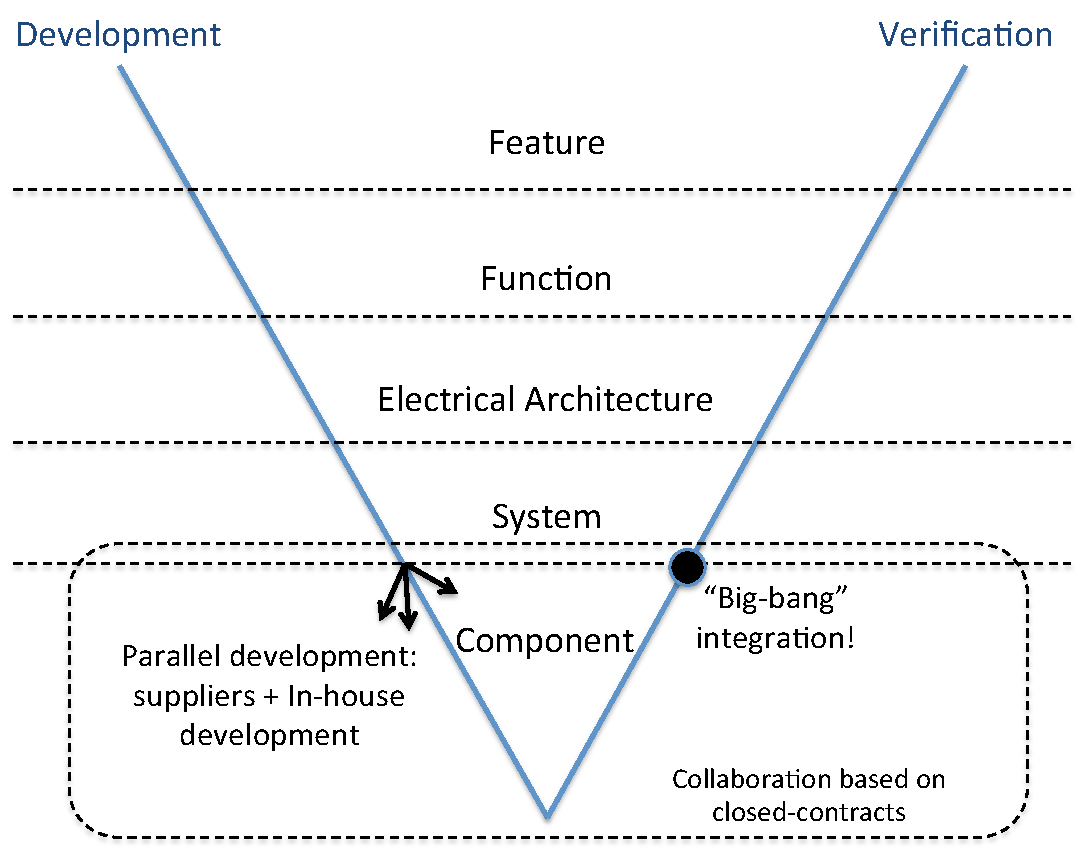
\includegraphics[width=.9\columnwidth]{figure/Closed-contract-collaboration.pdf}
%\vspace{-.2cm}
%\caption{Collaboration based on contracts\todo{Delete the figure}}
%\label{fig:closedContractCollaboration}
%\vspace{-.2cm}
%\end{figure}

Therefore, OEMs experience heavy reliance on external developers and subcontractors; this complicates coordination throughout the entire development process. Expensive communication and coordination delays during integration are results of outsourcing significant parts of development to suppliers. %This form of exponentially growing feature content severely complicates ``big-bang" integration~\cite{Eklund2012}. The development is inevitably parallelized; this obviously also holds for the large amount of externally developed software, which is integrated as black-box functionality~\cite{Patrizio2016AAF_Chalmers,Broy2009AAF_TUM,Broy:2006:CAS:1134285.1134292}. 


%\del{As shown in Figure~\ref{fig:closedContractCollaboration} the} \ins{
The software engineering process traditionally follows the V-model, %\chg{with the development on the left-hand side and verification on the right-hand side. The}{where} 
where development at the level of components is parallelized among the different suppliers, and internal in-house development. The degree of parallelism can easily reach level 50 (i.e. 50 parallel developments). Once the collaboration between the OEM and its suppliers is regulated by contract, parallel developments %\del{represented in Figure~\ref{fig:closedContractCollaboration}} 
start by signing a contract and  after months the large amount of externally developed software comes back to the OEM to be integrated as black-box functionality~\cite{Broy:2006:CAS:1134285.1134292}. 
%the produced ECUs will be provided back to the OEM after some months with few communication during the production period.
This leads to a challenging, complex, and sometimes chaotic integration. %: the developed Electronic Control Units (ECUs) (which include both hardware and software) come back to the OEM and integration starts. 
%It is a
At this stage %that 
many misunderstandings, conflicting interpretations, wrong assumptions, etc. are discovered.
%It is easy to understand 
Consequently, %that 
contract relations between the OEM and the suppliers might slow down the inter-organizational CI\&D.  %\todo{this last statement is disconnected from the rest of the story: miss the link between the mentioned integration problems and closed contracts}

%\todo{Show how CI\&D is implemented in automotive set-ups.}

%The collaboration between the stakeholders in the ecosystem needs to improve the software quality and provide faster, cheaper, and more predictable development~\cite{herbsleb2016IntelligentTransparent}. 
%
%This implies that the automotive (software) industry must identify how this new scenario\todo{what is the new scenario?} can be supported at best when an ecosystem of organizations collaborates.
%
%\todo{there is a gap between these two paragraphs: collaboration should be supported by new tools, like views and associated viewpoints to communicate the right architectural knowledge, etc.}
%
%These considerations motivate the need of considering new types of viewpoints and views\todo{add citation} from the perspective of specific system concerns, which are relevant for one or more stakeholders collaborating in the automotive ecosystem. Because of this, it is necessary for members of this ecosystem to agree on a common way of structuring\todo{what do you mean? structuring what?} in order to increase overall efficiency within the ecosystem \cite{Patrizio2016AAF_Chalmers,Broy2009AAF_TUM,Broy:2006:CAS:1134285.1134292}. An essential technical problem to solve for this vision is the establishment of standards for interoperability among IPs, both software and hardware, and tools \cite{Broy:2006:CAS:1134285.1134292}. ``Establishing and evolving ecosystems of different partner types might ultimately decide which companies win a market." \cite{Bosch2016Ecosystem}. First attempts, such as AUTOSAR \cite{acm2008autosar} and the Automotive Architecture Framework (AAF) \cite{Patrizio2016AAF_Chalmers,Broy2009AAF_TUM} are being developed. However, researchers and practitioners both identified the need for further research on this emerging type of software ecosystems.
%

In order to avoid such integration problems, automotive software development increasingly embraces continuous integration. 
Changes are implemented, locally tested, and then integrated into a main branch with the goal to obtain feedback from system level tests.
This way of working is now widely used by in house software teams that are working on software components.
Through submitting small changes early and often as well as fixing potential integration problems directly, quality and cycle time of changes can be improved.
But in order to benefit from these aspects on a system level, continuous integration from many teams need to be considered in a hierarchy of sub-systems.
In addition, software components that are developed in house often depend on other software components (e.g. basic software, runtime environments), developed by suppliers. 
Thus, it becomes increasingly important to understand how continuous integration can be supported when involving external organizations.

\ins{Standards, such as AUTOSAR, which defines a standard software architecture for electronic control units (ECU) \cite{fennel2006achievements}.
In the context of AUTOSAR, the following CI\&D scenario is not uncommon: 
The OEM develops AUTOSAR compatible application software components in-house in order to support functions in the car. 
These application software components rely on the runtime environment defined by AUTOSAR and provided through deliveries of the ECU hardware, AUTOSAR's basic software component, and special drivers by multiple suppliers.
Usually, one of these suppliers is responsible for integrating hardware, basic software components, and application components.
Note, that this external integration can cause delays in continuous integration.
Also note, that even in case of in-house integration, all software components (basic and application SW) need to be compiled into one binary that then is uploaded to the ECU.
}

\ins{The AUTOSAR consortium is currently working on a new flavour of AUTOSAR: Adaptive AUTOSAR.
In adaptive AUTOSAR, software components can be exchanged individually without recompiling the complete binary for the ECU.
Thus, an OEM could order a first version of ECU hardware and basic software, then iteratively integrate  several versions of their application software, learn limitations of the suppliers’ first delivery and use this knowledge for ordering future versions of hardware and basic software.
This scenario is made complicated by the fact that no upfront knowledge about the functionality of an integrated version is available.
Thus, integration tests need to be more dynamic as well, and functionality that is distributed over several ECUs does either not fully benefit from continuous integration (since all expected functionality needs to be implemented by all ECUs) or needs to rely on automated service discovery.}
 
\ins{In conclusion, despite these exciting developments with respect to standards, we foresee that system level CI\&D will have to rely on improved communication between OEM and supplier.
For this reason, we provide with this paper a first step to investigate transparency in the context of system level, cross-organizational, continuous integration.}